\subsection{Rapid Growth Requires an Increase in Ribosomal Copy Number and Cell Size}
% The relationship between cell size and growth rate has long been of interest in
% the study of bacterial physiology, particularly following the now six decade-old
% observation that cell volume appears to increase exponentially with growth rate;
% known as Schaechter's growth law \citep{schaechter1958, taheriaraghi2015}.
% However, the mechanism that governs this relationship, and even the question of
% whether the change in average cell size is truly exponential, has remained under
% debate \citep{harris2018}.  Here we examine the influence of ribosomal content
% and total protein abundance on cell size.

% though the simple addition of more ribosomes is likely constrained by aspects
% physical constraints like macromolecular crowding \citep{delarue2018,
% solerbistue2020}.

In \FIG{ribosome_limit}(C) we find that above about  0.75 hr$^{-1}$, the growth
rate is dictated by the ribosomal mass fraction $\Phi_R$, since $f_a$ is close
to 1, and $r_t$ is near its maximal rate [cite and refer to figure/
supplemental]. While the preceeding section helps us understand that cells will
need to increase $\Phi_R$ in order to grow faster, the fractional dependence
gives little insight into how this is actually achieved in the cell. Here we
consider the changes in absolute protein content and cell volume to better
understand how they relate to the dependence between growth rate and $\Phi_R$.

It is now well-documented that \textit{E. coli} cells add a constant volume per
origin of replication, which is robust to a remarkable array of cellular
perturbations \citep{si2017}.  The average number of origins per cell, $\langle$\#
ori$\rangle$, is set by how often replication must be initiated per cell doubling
under steady-state growth. This can be quantified as
\begin{equation}
    \langle \text{\# ori} \rangle = 2^{\tau_{cyc} / \tau} = 2^{\tau_{cyc} \lambda / ln(2)},
    \label{eq:Nori}
\end{equation}
where $t_{cyc}$ is the cell cycle time (referring to the time from replication
initiation to cell division), and $\tau$ is the cell doubling time. To consider
this  in the context of the proteomic data, we used measurements of $\tau_{cyc}$
and  $\tau$ from \cite{si2017} (\FIG{translation_ecoli_partA}(A)) to estimate
the calculate $\langle$\# ori$\rangle$  with \EQ{Nori} at different growth
rates. For ribosomal synthesis, we find an approximately linear correlation
between ribosome copy number and $\langle$\# ori$\rangle$
(\FIG{translation_ecoli_partA}(B)).

For a constant cell cycle time, which is observed at growth rates above about
0.5 hr$^{-1}$ (\FIG{translation_ecoli_partA}(A), \citep{helmstetter1968}),
\EQ{Nori} states that $\langle \text{\# ori} \rangle$ will need to increase
exponentially with the growth rate. While this says nothing of the observed
scaling between cell size and growth rate, the additional dependency on
ribosomal fraction through \EQ{translation_limit_growth_rate} provides an
important link. To better explore how cells vary protein abundance proteome-wide
across growth conditions, in \FIG{translation_ecoli_partA}(D), we
determined the position-dependent protein expression across the chromosome by
calculating a running Gaussian average of protein copy number (20 kbp st. dev.
averaging window) based on each gene's transcriptional start site. These were
median-subtracted to account for the differences in total protein abundance.
Importantly, the major deviations in protein copy number are largely restricted to
regions of ribosomal protein genes. This suggests that the ribosomal fraction
$\Phi_R$ is also being tuned in proportion to $\langle$\# ori$\rangle$, and that
it is through this dependence that \textit{E. coli} exhibits an exponential
increase in cell volume with growth rate.

\begin{figure*}
    \begin{fullwidth}
    \centering{
        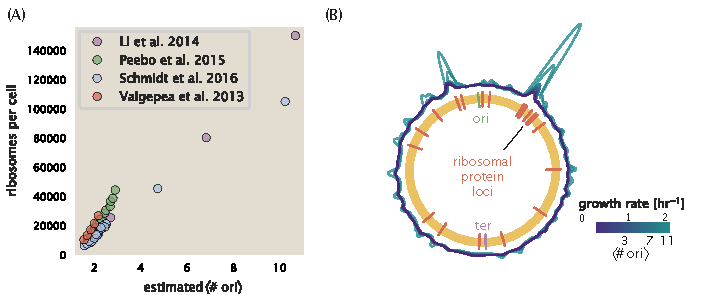
\includegraphics{main_figs/fig8_ribosome_growth_limit_ecoli_a_polar_coord.pdf}
        \caption{\textbf{Cells increase absolute ribosome abundance with
        $\langle$\# ori$\rangle$.} (A) Experimental measurements of
        the cell doubling time $\tau$ and cell cycle time $t_{cyc}$
         from Si \textit{et al.}
        (2017). Dashed line shows fit to the data, which were used to estimate
        $\langle$\# ori$\rangle$. $t_{cyc}$ was assumed to vary in proportion to
        $\tau$ for doubling times greater than 40 minutes, and reach a
        minimum value of 73 minutes (see Appendix
        \nameref{sec:SI_ori} for additional details). Red data points correspond
        to measurements in strain MG1655, while light green points are for
        strain NCM3722. (B) Plot of the ribosome copy number estimated from the
        proteomic data against the estimated $\langle$\# ori$\rangle$. (C)
        Schematic shows the expected increase in replication forks (or number of
        ori regions) as \textit{E. coli} cells grow faster. (D) A running
        Gaussian average (20 kbp st. dev.) of protein copy number is calculated
        for each growth condition considered by \citep{schmidt2016}. Since total
        protein abundance increases with growth rate, protein copy numbers are
        median-subtracted to allow comparison between growth conditions.
        $\langle$\# ori$\rangle$ are estimated using the data in (A) and
        Equation \ref{eq:Nori}. } \label{fig:translation_ecoli_partA}
    }
    \end{fullwidth}
\end{figure*}
